\documentclass[11pt,a4paper]{report}
\usepackage[textwidth=37em,vmargin=30mm]{geometry}
\usepackage{calc,xunicode,amsmath,amssymb,paralist,enumitem,tabu,booktabs,datetime2,xeCJK,xeCJKfntef,listings}
\usepackage{tocloft,fancyhdr,tcolorbox,xcolor,graphicx,eso-pic,xltxtra,xelatexemoji}

\newcommand{\envyear}[0]{2025}
\newcommand{\envdatestr}[0]{2025-08-18}
\newcommand{\envfinaldir}[0]{webdb/2025/20250818/final}

\usepackage[hidelinks]{hyperref}
\hypersetup{
    colorlinks=false,
    pdfpagemode=FullScreen,
    pdftitle={Web Digest - \envdatestr}
}

\setlength{\cftbeforechapskip}{10pt}
\renewcommand{\cftchapfont}{\rmfamily\bfseries\large\raggedright}
\setlength{\cftbeforesecskip}{2pt}
\renewcommand{\cftsecfont}{\sffamily\small\raggedright}

\setdefaultleftmargin{2em}{2em}{1em}{1em}{1em}{1em}

\usepackage{xeCJK,xeCJKfntef}
\xeCJKsetup{PunctStyle=plain,RubberPunctSkip=false,CJKglue=\strut\hskip 0pt plus 0.1em minus 0.05em,CJKecglue=\strut\hskip 0.22em plus 0.2em}
\XeTeXlinebreaklocale "zh"
\XeTeXlinebreakskip = 0pt


\setmainfont{Brygada 1918}
\setromanfont{Brygada 1918}
\setsansfont{IBM Plex Sans}
\setmonofont{JetBrains Mono NL}
\setCJKmainfont{Noto Serif CJK SC}
\setCJKromanfont{Noto Serif CJK SC}
\setCJKsansfont{Noto Sans CJK SC}
\setCJKmonofont{Noto Sans CJK SC}

\setlength{\parindent}{0pt}
\setlength{\parskip}{8pt}
\linespread{1.15}

\lstset{
	basicstyle=\ttfamily\footnotesize,
	numbersep=5pt,
	backgroundcolor=\color{black!5},
	showspaces=false,
	showstringspaces=false,
	showtabs=false,
	tabsize=2,
	captionpos=b,
	breaklines=true,
	breakatwhitespace=true,
	breakautoindent=true,
	linewidth=\textwidth
}






\newcommand{\coverpic}[2]{
    % argv: itemurl, authorname
    Cover photo by #2~~(\href{#1}{#1})
}
\newcommand{\makeheader}[0]{
    \begin{titlepage}
        % \newgeometry{hmargin=15mm,tmargin=21mm,bmargin=12mm}
        \begin{center}
            
            \rmfamily\scshape
            \fontspec{BaskervilleF}
            \fontspec{Old Standard}
            \fontsize{59pt}{70pt}\selectfont
            WEB\hfill DIGEST
            
            \vfill
            % \vskip 30pt
            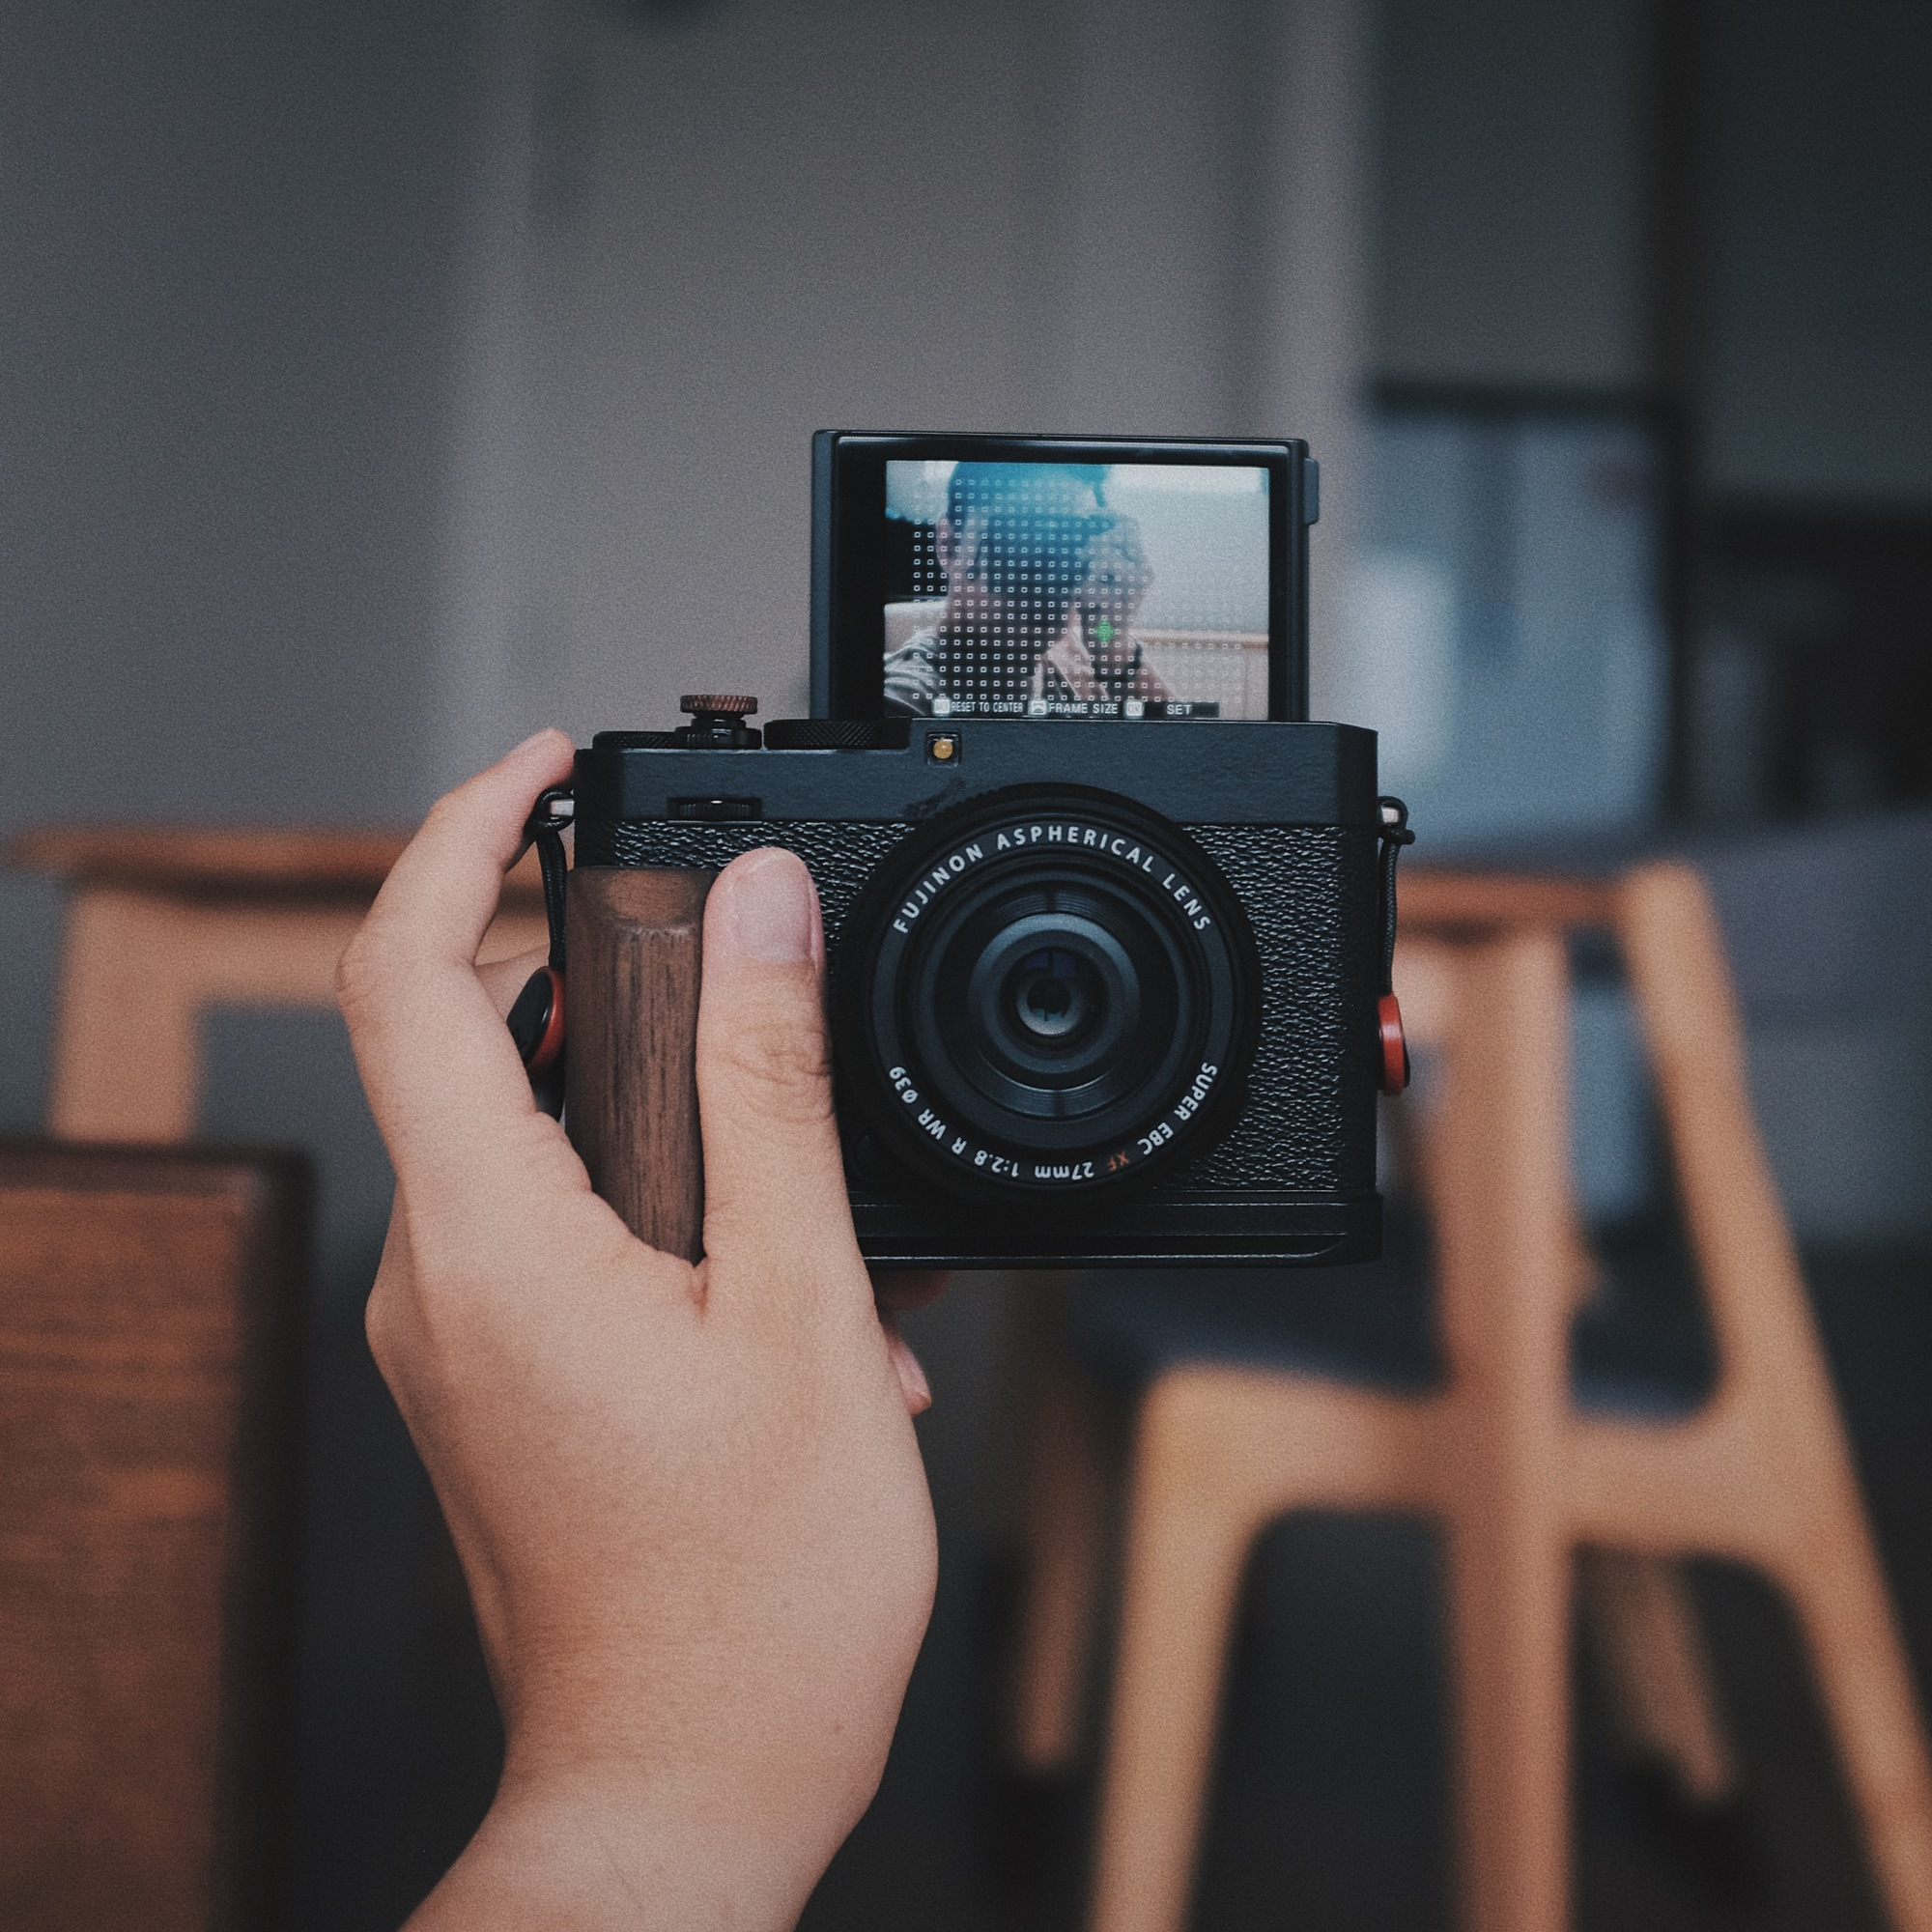
\includegraphics[width=\linewidth]{\envfinaldir/coverpic-prod.jpg}\par
            % \vskip 30pt
            \vfill

            \normalsize\rmfamily\scshape
            \copyright{} The Web Digest Project \hfill\large \envdatestr
        \end{center}
    \end{titlepage}
    % \restoregeometry
}
\newcommand{\simplehref}[1]{%
    \textcolor{blue!80!green}{\href{#1}{#1}}%
}
\renewcommand{\contentsname}{\center\Huge\sffamily\bfseries Contents\par\vskip 20pt}
\newcounter{ipartcounter}
\setcounter{ipartcounter}{0}
\newcommand{\ipart}[1]{
    % \vskip 20pt
    \clearpage
    \stepcounter{ipartcounter}
    \phantomsection
    \addcontentsline{toc}{chapter}{#1}
    % \begin{center}
    %     \Huge
    %     \sffamily\bfseries
    %     #1
    % \end{center}
    % \vskip 20pt plus 7pt
}
\newcounter{ichaptercounter}
\setcounter{ichaptercounter}{0}
\newcommand{\ichapter}[1]{
    % \vskip 20pt
    \clearpage
    \stepcounter{ichaptercounter}
    \phantomsection
    \addcontentsline{toc}{section}{\numberline{\arabic{ichaptercounter}}#1}
    \begin{center}
        \Huge
        \sffamily\bfseries
        #1
    \end{center}
    \vskip 20pt plus 7pt
}
\newcommand{\entrytitlefont}[1]{\subsection*{\raggedright\Large\sffamily\bfseries#1}}
\newcommand{\entryitemGeneric}[2]{
    % argv: title, url
    \parbox{\linewidth}{
        \entrytitlefont{#1}\par\vskip 5pt
        \footnotesize\ttfamily\mdseries
        \simplehref{#2}
    }\vskip 11pt plus 11pt minus 1pt
}
\newcommand{\entryitemGithub}[3]{
    % argv: title, url, desc
    \parbox{\linewidth}{
        \entrytitlefont{#1}\par\vskip 5pt
        \footnotesize\ttfamily\mdseries
        \simplehref{#2}\par\vskip 5pt
        \small\rmfamily\mdseries#3
    }\vskip 11pt plus 11pt minus 1pt
}
\newcommand{\entryitemAp}[3]{
    % argv: title, url, desc
    \parbox{\linewidth}{
        \entrytitlefont{#1}\par\vskip 5pt
        \footnotesize\ttfamily\mdseries
        \simplehref{#2}\par\vskip 5pt
        \small\rmfamily\mdseries#3
    }\vskip 11pt plus 11pt minus 1pt
}
\newcommand{\entryitemHackernews}[3]{
    % argv: title, hnurl, rawurl
    % \parbox{\linewidth}{
    %     \entrytitlefont{#1}\par\vskip 5pt
    %     \footnotesize\ttfamily\mdseries
    %     \simplehref{#3}\par
    %     \textcolor{black!50}{\href{#2}{#2}}
    % }\vskip 11pt plus 11pt minus 1pt
    \begin{minipage}{\linewidth}
            \entrytitlefont{#1}\par\vskip 5pt
            \footnotesize\ttfamily\mdseries
            \simplehref{#3}\par
            \textcolor{black!50}{\href{#2}{#2}}
    \end{minipage}\par\vskip 11pt plus 11pt minus 1pt
}







\begin{document}

\makeheader

\tableofcontents\clearpage




\ipart{Developers}
\ichapter{Hacker News}
\entryitemTwoLinks{Claude Opus 4 and 4.1 can now end a rare subset of conversations}{https://news.ycombinator.com/item?id=44916813}{https://www.anthropic.com/research/end-subset-conversations}

\entryitemTwoLinks{Imagen 4 is now generally available}{https://news.ycombinator.com/item?id=44915187}{https://developers.googleblog.com/en/announcing-imagen-4-fast-and-imagen-4-family-generally-available-in-the-gemini-api/}

\entryitemTwoLinks{Show HN: Edka – Kubernetes clusters on your own Hetzner account}{https://news.ycombinator.com/item?id=44915164}{https://edka.io}

\entryitemTwoLinks{It seems like the AI crawlers learned how to solve the Anubis challenges}{https://news.ycombinator.com/item?id=44914773}{https://social.anoxinon.de/@Codeberg/115033790447125787}

\entryitemTwoLinks{Steam can't escape the fallout from its censorship controversy}{https://news.ycombinator.com/item?id=44914163}{https://www.polygon.com/steam-paypal-issues-censorship-visa-mastercard/}

\entryitemTwoLinks{Occult books digitized and put online by Amsterdam's Ritman Library}{https://news.ycombinator.com/item?id=44914061}{https://www.openculture.com/2025/08/2178-occult-books-now-digitized-put-online.html}

\entryitemTwoLinks{The electric fence stopped working years ago}{https://news.ycombinator.com/item?id=44913663}{https://soonly.com/electric-fences/}

\entryitemTwoLinks{Do Things That Don't Scale (2013)}{https://news.ycombinator.com/item?id=44913359}{https://paulgraham.com/ds.html}

\entryitemTwoLinks{The beauty of a text only webpage}{https://news.ycombinator.com/item?id=44913340}{https://albanbrooke.com/the-beauty-of-a-text-only-webpage/}

\entryitemTwoLinks{ADHD drug treatment and risk of negative events and outcomes}{https://news.ycombinator.com/item?id=44912861}{https://www.bmj.com/content/390/bmj-2024-083658}

\entryitemTwoLinks{The Timmy Trap}{https://news.ycombinator.com/item?id=44912646}{https://jenson.org/timmy/}

\entryitemTwoLinks{White House loyalty rating for companies}{https://news.ycombinator.com/item?id=44912369}{https://www.axios.com/2025/08/15/white-house-rating-big-beautiful-bill}

\entryitemTwoLinks{Is Germany on the brink of banning ad blockers?}{https://news.ycombinator.com/item?id=44912085}{https://blog.mozilla.org/netpolicy/2025/08/14/is-germany-on-the-brink-of-banning-ad-blockers-user-freedom-privacy-and-security-is-at-risk/}

\entryitemTwoLinks{Vaultwarden commit introduces SSO using OpenID Connect}{https://news.ycombinator.com/item?id=44911560}{https://github.com/dani-garcia/vaultwarden/pull/3899}

\entryitemTwoLinks{Open hardware desktop 3D printing is dead?}{https://news.ycombinator.com/item?id=44911423}{https://www.josefprusa.com/articles/open-hardware-in-3d-printing-is-dead/}

\entryitemTwoLinks{Fairness is what the powerful 'can get away with' study shows}{https://news.ycombinator.com/item?id=44911169}{https://phys.org/news/2025-07-fairness-powerful.html}

\entryitemTwoLinks{Court records reveal Sig Sauer knew of pistol risks for years}{https://news.ycombinator.com/item?id=44911069}{https://smokinggun.org/court-records-reveal-sig-sauer-knew-of-pistol-risks-for-years/}

\entryitemTwoLinks{Swiss vs. UK approach to major tranport projects}{https://news.ycombinator.com/item?id=44910393}{https://www.freewheeling.info/blog/swiss-hs2}

\entryitemTwoLinks{UK government states that 'safety' act is about influence over public discourse}{https://news.ycombinator.com/item?id=44910161}{https://bsky.app/profile/tupped.bsky.social/post/3lwgcmswmy222}

\entryitemTwoLinks{Simulating and Visualising the Central Limit Theorem}{https://news.ycombinator.com/item?id=44909133}{https://blog.foletta.net/post/2025-07-14-clt/}\ichapter{Phoronix}
\entryitemGeneric{\hskip 0pt{}Linux 6.17-rc2 Released With Performance Fixes \& More}{https://www.phoronix.com/news/Linux-6.17-rc2-Released}

\entryitemGeneric{\hskip 0pt{}Linux 6.17 Performance Looking Even Better After Early Fallout Addressed}{https://www.phoronix.com/news/Linux-6.17-Benchmarks-Round-2}

\entryitemGeneric{\hskip 0pt{}Linux 6.17-rc2 To Better Tune Attack Vector Controls For SRSO Mitigation}{https://www.phoronix.com/news/Linux-6.17-rc2-Tune-Attack-Vec}

\entryitemGeneric{\hskip 0pt{}Linux Merges Headset Detection Workaround For Framework 13 Ryzen AI 300 Series}{https://www.phoronix.com/news/Framework-13-AI-300-Headset}

\entryitemGeneric{\hskip 0pt{}Shotcut 25.08 Brings More Bug Fixes To This Open-Source Video Editor}{https://www.phoronix.com/news/Shotcut-25.08-Released}

\entryitemGeneric{\hskip 0pt{}Fedora Copr Repository Offers XLibre Packages For Alternative X Server}{https://www.phoronix.com/news/Fedora-XLibre-Copr-Repo}

\entryitemGeneric{\hskip 0pt{}Linux 6.16.1 Fixes A Large Intel GPU Driver Performance Regression - Up To 30\%}{https://www.phoronix.com/news/Linux-6.16.1-Fixes-Intel-i915}

\entryitemGeneric{\hskip 0pt{}GNOME Disks Continues Being Ported To Rust}{https://www.phoronix.com/news/GNOME-Disks-More-Rust}

\entryitemGeneric{\hskip 0pt{}Wine-Staging 10.13 Adds Patch For 13 Year Old Bug}{https://www.phoronix.com/news/Wine-Staging-10.13}


\ipart{Developers~~~~(zh-Hans)}
\ichapter{Solidot}
\entryitemGeneric{\hskip 0pt{}克罗地亚将数字游民签证有效期延长至三年}{https://www.solidot.org/story?sid=82067}

\entryitemGeneric{\hskip 0pt{}今年前七个月电动汽车销量同比增长 27\%}{https://www.solidot.org/story?sid=82066}

\entryitemGeneric{\hskip 0pt{}PuTTY 有了新官网}{https://www.solidot.org/story?sid=82065}

\entryitemGeneric{\hskip 0pt{}德国最高法院部分推翻广告屏蔽工具不侵犯版权判决}{https://www.solidot.org/story?sid=82064}

\entryitemGeneric{\hskip 0pt{}维基百科历史上最大规模的自我推销行动}{https://www.solidot.org/story?sid=82063}

\entryitemGeneric{\hskip 0pt{}Google 发布紧凑型开源模型 Gemma 3 270M}{https://www.solidot.org/story?sid=82062}

\entryitemGeneric{\hskip 0pt{}退休后继续工作与更高的幸福度相关}{https://www.solidot.org/story?sid=82061}

\entryitemGeneric{\hskip 0pt{}半人马座 α 星可能存在一颗气态巨行星}{https://www.solidot.org/story?sid=82060}

\entryitemGeneric{\hskip 0pt{}特朗普政府考虑入股英特尔}{https://www.solidot.org/story?sid=82059}

\entryitemGeneric{\hskip 0pt{}现阶段的印度越南制造还只是中国加一}{https://www.solidot.org/story?sid=82058}

\entryitemGeneric{\hskip 0pt{}微软高管称语音将成为下一代 Windows 的主要输入方式}{https://www.solidot.org/story?sid=82057}

\entryitemGeneric{\hskip 0pt{}一氧化碳新解毒剂能在数分钟内清理血液}{https://www.solidot.org/story?sid=82056}

\entryitemGeneric{\hskip 0pt{}AI 数据中心推动美国居民电费全面上涨}{https://www.solidot.org/story?sid=82055}

\entryitemGeneric{\hskip 0pt{}广岛和长崎核爆幸存者死于辐射致癌的比例比预期的低}{https://www.solidot.org/story?sid=82054}

\entryitemGeneric{\hskip 0pt{}ReiserFS 在内核的最后残余被清除}{https://www.solidot.org/story?sid=82053}\ichapter{V2EX}
\entryitemGeneric{\hskip 0pt{}[奇思妙想] 虚拟角色聊天似乎还有机会,要不要做}{https://www.v2ex.com/t/1153042}

\entryitemGeneric{\hskip 0pt{}[游戏] 有玩战地 6 的朋友吗}{https://www.v2ex.com/t/1153041}

\entryitemGeneric{\hskip 0pt{}[程序员] Any Router 挂啦?注册好还没用过呢。}{https://www.v2ex.com/t/1153040}

\entryitemGeneric{\hskip 0pt{}[问与答] 新人报道,以及询问相关问题}{https://www.v2ex.com/t/1153038}

\entryitemGeneric{\hskip 0pt{}[Apple] 分享一个 JetBrains 全家桶在支持 Promotion 的 MacBook 上,滑动没有高刷效果的解决方案}{https://www.v2ex.com/t/1153037}

\entryitemGeneric{\hskip 0pt{}[程序员] 大佬们,有没有办法可以监控获取到钉钉群的消息}{https://www.v2ex.com/t/1153036}

\entryitemGeneric{\hskip 0pt{}[分享创造] 最近新上架了一个不需要 VPN 的 iOS Tailscale SSH Terminal 免费客户端}{https://www.v2ex.com/t/1153035}

\entryitemGeneric{\hskip 0pt{}[问与答] 有没有插件可以快速在 jetbrains 和 Cursor 之间切换}{https://www.v2ex.com/t/1153034}

\entryitemGeneric{\hskip 0pt{}[职场话题] 要不要跳槽的问题}{https://www.v2ex.com/t/1153033}

\entryitemGeneric{\hskip 0pt{}[Steam] Steam Deck 运行 pacman 指令疑似被投毒}{https://www.v2ex.com/t/1153032}

\entryitemGeneric{\hskip 0pt{}[问与答] 体验了一把运动小飞机低空飞行,感觉挺酷。}{https://www.v2ex.com/t/1153031}

\entryitemGeneric{\hskip 0pt{}[问与答] V 友们周末怎么过的呢,做个小调查}{https://www.v2ex.com/t/1153030}

\entryitemGeneric{\hskip 0pt{}[阅读] 求助 uvz 格式电子书阅读软件安卓版}{https://www.v2ex.com/t/1153028}

\entryitemGeneric{\hskip 0pt{}[分享创造] 用视觉大语言模型检索表情包}{https://www.v2ex.com/t/1153026}

\entryitemGeneric{\hskip 0pt{}[问与答] 现在国内有什么还可以用 claude 的 ide 方案吗}{https://www.v2ex.com/t/1153025}

\entryitemGeneric{\hskip 0pt{}[分享创造] 从 Claude Code 到 GrowBlank - 软件进化的新范式}{https://www.v2ex.com/t/1153024}

\entryitemGeneric{\hskip 0pt{}[分享创造] Chrome 离线翻译插件已上架 Chrome 扩展商店 一比一还原原生网页翻译}{https://www.v2ex.com/t/1153022}

\entryitemGeneric{\hskip 0pt{}[职场话题] 日本和越南,最近老是听说做 SAAS 在这两个国家缺口很大~想请教一下各位 V 友,事实真的是这样么?}{https://www.v2ex.com/t/1153021}

\entryitemGeneric{\hskip 0pt{}[分享发现] 记第一次上台展示}{https://www.v2ex.com/t/1153020}

\entryitemGeneric{\hskip 0pt{}[职场话题] 我第 2 次拒绝加班了}{https://www.v2ex.com/t/1153019}

\entryitemGeneric{\hskip 0pt{}[问与答] Fedora 42 使用 docker-compose 安装的 immich 无法用 ip 访问}{https://www.v2ex.com/t/1153016}

\entryitemGeneric{\hskip 0pt{}[分享创造] 为了爽看凡人修仙传,我花两天时间写了个知识图谱应用}{https://www.v2ex.com/t/1153014}

\entryitemGeneric{\hskip 0pt{}[摄影] 穴小鸮}{https://www.v2ex.com/t/1153013}

\entryitemGeneric{\hskip 0pt{}[问与答] 允许``微信''查找本地网络中的设备?}{https://www.v2ex.com/t/1153011}

\entryitemGeneric{\hskip 0pt{}[加密货币] 关于交易:我踩过的坑和我对交易的认知}{https://www.v2ex.com/t/1153010}

\entryitemGeneric{\hskip 0pt{}[Solana] 刚才扫链扫到个自毁网站 好像很久之前见过}{https://www.v2ex.com/t/1153009}

\entryitemGeneric{\hskip 0pt{}[NAS] 群晖 BTRFS 恢复求助.}{https://www.v2ex.com/t/1153008}

\entryitemGeneric{\hskip 0pt{}[分享创造] 用 beancount 记账的朋友进,写了一个用于生成港股通记录的工具。}{https://www.v2ex.com/t/1153007}

\entryitemGeneric{\hskip 0pt{}[奇思妙想] 如果烹饪流程能够标准化,能够还原出家庭餐厅的味道}{https://www.v2ex.com/t/1153006}

\entryitemGeneric{\hskip 0pt{}[投资] 有年化收益率 5~10\%低风险投资推荐吗}{https://www.v2ex.com/t/1153004}

\entryitemGeneric{\hskip 0pt{}[推广] 一万字讲透流量卡,避开所有的坑,为什么到处都是流量卡广告 [风无前]}{https://www.v2ex.com/t/1153003}

\entryitemGeneric{\hskip 0pt{}[分享创造] 开源了一个 AI 驱动基于 Tailwind CSS 的 React 组件库生成器}{https://www.v2ex.com/t/1153002}

\entryitemGeneric{\hskip 0pt{}[分享创造] 写了一个程序员版本的 16 型人格测试}{https://www.v2ex.com/t/1153001}

\entryitemGeneric{\hskip 0pt{}[PHP] 大家好,我又來了,新作品 https://www.freetalkhub.com, PHP 开发}{https://www.v2ex.com/t/1153000}

\entryitemGeneric{\hskip 0pt{}[VXNA] 今天(8/17)凌晨更新了一篇博客,但直到现在(7:30pm)仍然没有被聚合}{https://www.v2ex.com/t/1152999}

\entryitemGeneric{\hskip 0pt{}[问与答] 测试 EO 与 ESA 对比 CF,为什么 esa 那么拉垮?}{https://www.v2ex.com/t/1152997}

\entryitemGeneric{\hskip 0pt{}[分享创造] 分享一个苹果发布会形式的 HTML PPT 模板,用来做研发工作汇报}{https://www.v2ex.com/t/1152996}

\entryitemGeneric{\hskip 0pt{}[投资] a 股已经明确是牛市,说下个人的观点}{https://www.v2ex.com/t/1152995}

\entryitemGeneric{\hskip 0pt{}[职场话题] 国内大厂前端/全栈 的 junior 岗位都是什么人在做?}{https://www.v2ex.com/t/1152994}

\entryitemGeneric{\hskip 0pt{}[OpenWrt] 再也不折腾旁路由了, FQ 的尽头还是客户端}{https://www.v2ex.com/t/1152993}

\entryitemGeneric{\hskip 0pt{}[职场话题] 如何从程序员成长为产品经理?自从用 AI 帮写代码,有时间思考了,也发现自己缺少产品直觉}{https://www.v2ex.com/t/1152992}

\entryitemGeneric{\hskip 0pt{}[酷工作] 招兼职前端 APP 电子书阅读器的开发}{https://www.v2ex.com/t/1152991}

\entryitemGeneric{\hskip 0pt{}[职场话题] 申请换组被告密,应该何去何从:半年前的热帖更新后续}{https://www.v2ex.com/t/1152990}

\entryitemGeneric{\hskip 0pt{}[生活] 夏天洗个头,头发会湿两次:洗完湿一次,吹完出汗湿一次}{https://www.v2ex.com/t/1152988}

\entryitemGeneric{\hskip 0pt{}[生活] [生活] 卖房子遇``装修代卖''有何套路?}{https://www.v2ex.com/t/1152987}

\entryitemGeneric{\hskip 0pt{}[问与答] 请问海康的 4200 客户端数据有办法同步么}{https://www.v2ex.com/t/1152986}

\entryitemGeneric{\hskip 0pt{}[程序员] 韩老魔昨天结婴了!为了本地欣赏老魔结婴过程,修复了一个 B 站会员视频下载器}{https://www.v2ex.com/t/1152985}

\entryitemGeneric{\hskip 0pt{}[iPhone] 这个``失窃设备保护''到底怎么关闭?}{https://www.v2ex.com/t/1152983}

\entryitemGeneric{\hskip 0pt{}[酷工作] 前端工程师(React 方向)丨深圳招聘线下全职}{https://www.v2ex.com/t/1152982}

\entryitemGeneric{\hskip 0pt{}[iPhone] iOS26 的截图功能是不是颜色有点偏差?}{https://www.v2ex.com/t/1152981}


\ipart{Generic News}







\clearpage
\leavevmode\vfill
\footnotesize

Copyright \copyright{} 2023-2025 Neruthes and other contributors.

This document is published with CC BY-NC-ND 4.0 license.

The entries listed in this newsletter may be copyrighted by their respective creators.

This newsletter is generated by the Web Digest project.

The newsletters are also delivered via Telegram channel \CJKunderline{\href{https://t.me/webdigestchannel}{https://t.me/webdigestchannel}}.\\
RSS feed is available at \CJKunderline{\href{https://webdigest.pages.dev/rss.xml}{https://webdigest.pages.dev/rss.xml}}.

This newsletter is available in PDF at
\CJKunderline{\href{https://webdigest.pages.dev/}{https://webdigest.pages.dev/}}.

The source code being used to generate this newsletter is available at\\
\CJKunderline{\href{https://github.com/neruthes/webdigest}{https://github.com/neruthes/webdigest}}.

This newsletter is also available in
\CJKunderline{\href{http://webdigest.pages.dev/readhtml/\envyear/WebDigest-20250818.html}{HTML}} and
\CJKunderline{\href{https://github.com/neruthes/webdigest/blob/master/markdown/\envyear/WebDigest-20250818.md}{Markdown}}.


\coverpic{https://unsplash.com/photos/stone-castle-on-the-water-with-a-sailboat-U46FBFiJb-A}{Ana-Maria Stancu}


\end{document}
